\chapter{Our Approach}
\label{sec:our-approach}

\section{System Architecture}
% Brief introdcution of all actors, components and messages
% The specification is complicated because it is the result of long discussions and a clarification process (See https://project.redbackup.org/browse/REDPRO-98)
% See Describing architectures in https://wiki.hsr.ch/FarhadMehta/files/Writing_Scientific_Papers.pdf
% Describe everything concise and with exact definitions.
% Use schemes and flowcharts

There are two kinds of actors interacting with the system. A typical \gls{user} wants to store backups in the redbackup system and restore them (partially) when needed. The other kind of actor is an \gls{administrator} that configures the system, e.g. extends storage capacity or replaces corrupted disks. Distinctive for both actors is that they do not want to interact directly with the system unless human interaction is inevitable. This takes the burden to create backups manually from the user including the risk of oblivion and minimises management efforts required by the administrator.  Both actors, as well as their intentions, are described in more detail in Appendix \fullref{sec:specification}. Figure \ref{fig:c4-overview} presents a high-level overview that illustrates the interactions of the actors with the redbackup system.

\begin{figure}[h]
	\centering
	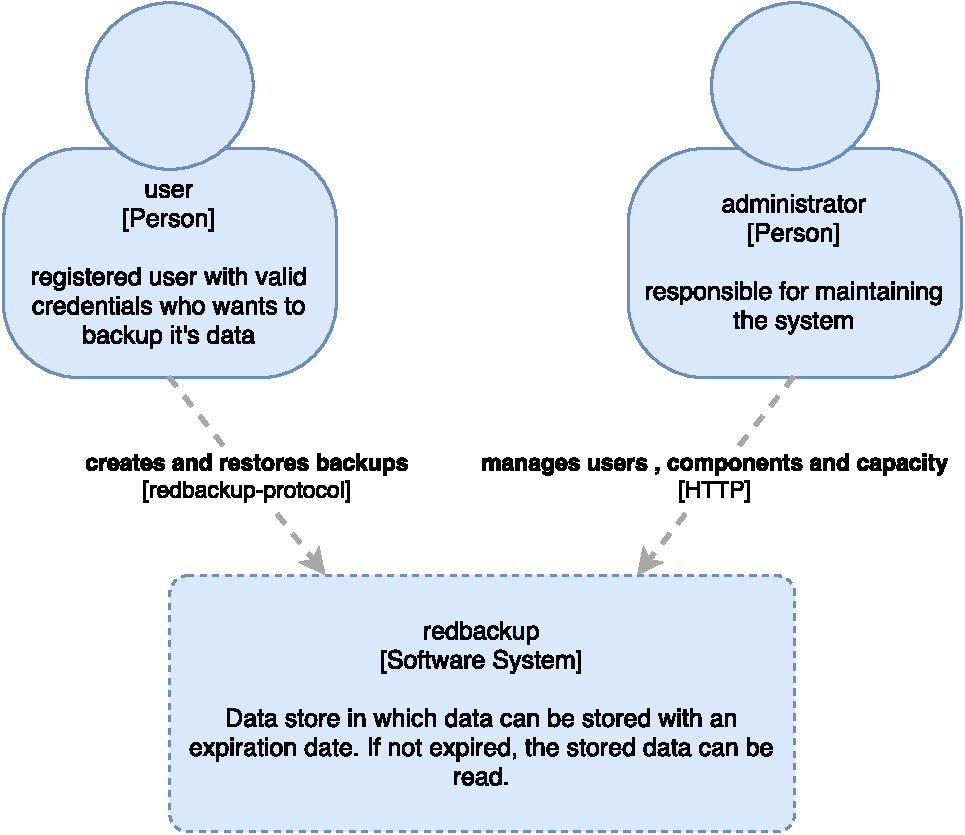
\includegraphics[width=0.5\linewidth]{resources/c4-overview}
	\caption[C4 System Context diagram]{C4 System Context diagram showing the big picture}
	\label{fig:c4-overview}
\end{figure}

The redbackup system consists of four core components as shown in the C4 Container diagram in Figure \ref{fig:c4-container}. A \gls{user} instructs a \gls{client} program running typically on the users machine to perform (unattended) backups and restores.  A client persists and loads its data from one or more interconnected \glspl{node}. A \gls{node} then is in charge of the data and its replication onto other nodes. \Glspl{node} persist the actual data in a separate component, a gls{storage}, to encapsulate persistence from replication and interaction to support different kinds of storage technologies (e.g. plain file systems or databases). A \gls{node} and its \gls{storage} are typically deployed on the same host. One central \gls{management} component orchestrates the configuration of the system by providing metadata, to clients and nodes. This metadata includes a set of all nodes in the system including their addresses and states,  user information and more. Clients and nodes can cache this metadata which ensures that a temporary unavailability of the management component does not compromise the replication and backup process. All components including their responsibilities and interactions are described in more detail in Appendix \fullref{sec:specification}.

\begin{figure}[h]
	\centering
	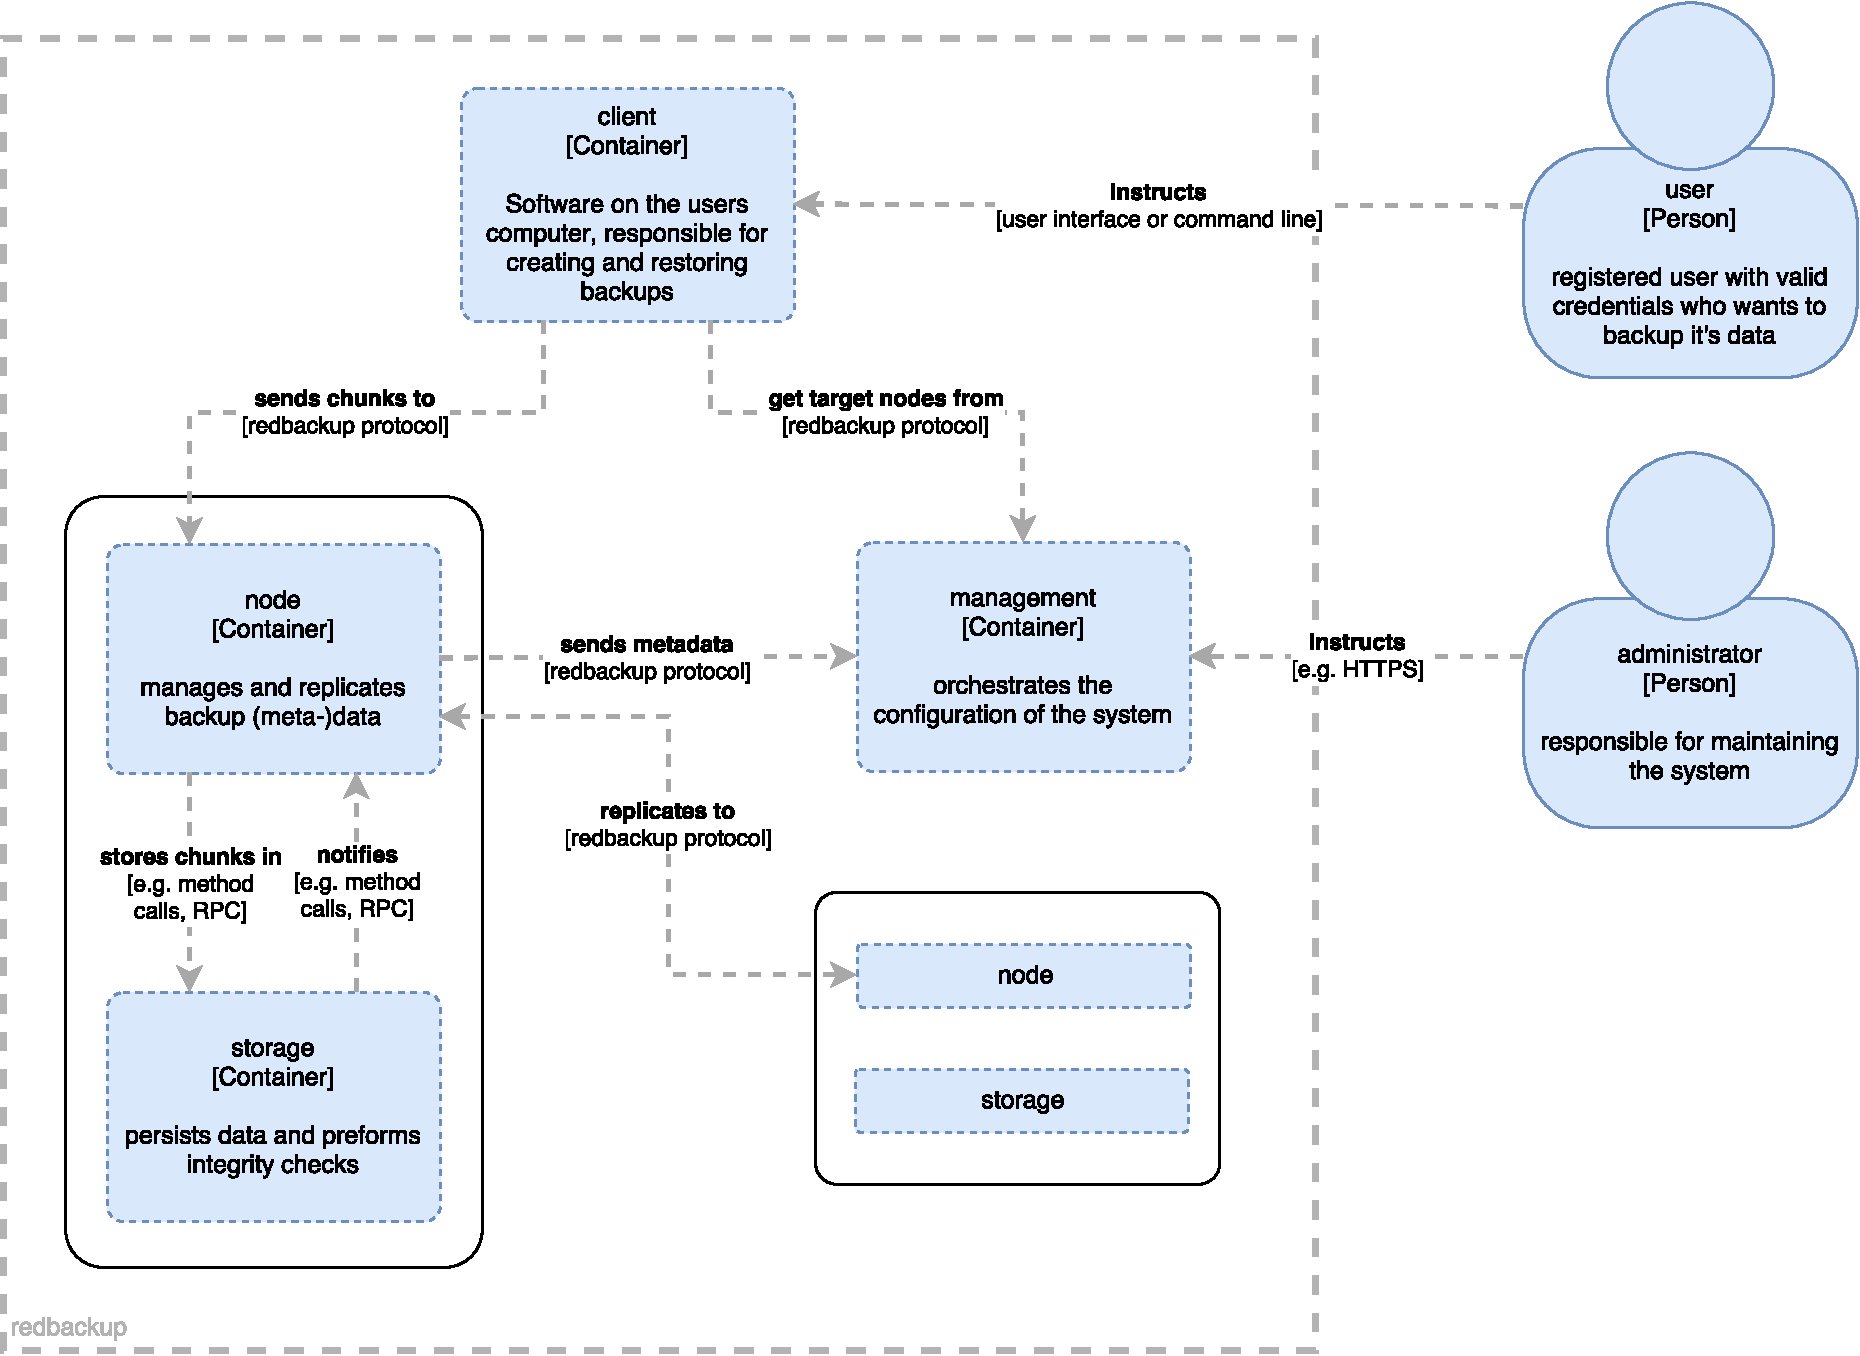
\includegraphics[width=1\linewidth]{resources/c4-container}
	\caption[C4 Container diagram]{C4 Container diagram illustrating the high-level shape of the redbackup software system and how responsibilities are distributed across it.}
	\label{fig:c4-container}
\end{figure}

Redbackup specifies a high-level protocol that is used for internal communication (noted in all C4 diagrams as \emph{redbackup protocol}). We deliberately specified the communication on a high level to encapsulate the underlying protocol. In the prototype, we used a custom, minimal protocol that is based on TCP and sends framed Message Pack\footnote{\url{https://msgpack.org/}} encoded messages. We also encapsulated the (de-) serialisation mechanisms in forwarder and receiver components as specified in the Forwarder Receiver Pattern Pattern \cite{POSA1}.  If we decided to switch to HTTP as the underlying protocol in the future, e.g. to overcome firewall issues, only these forwarder and receiver components have to be adapted while the actual message format does not change. 

\subsection{Replication}
% Planned and unplanned leaving of nodes
% Management down

As for this study project, we only specified n-replication (See \fullref{sec:fundamental-design-decisions}) because it is the most straightforward strategy to implement. A \gls{node} is in charge for all data stored on it. Each \gls{node} - hereafter called \gls{sending-node} -  picks $n$ random data \glspl{chunk} that are stored on it. It then randomly picks one other \gls{node} - hereafter called \gls{designated-node} - and requests which of the chosen data \glspl{chunk} are persisted on it. The \gls{designated-node} returns a subset of the requested \glspl{chunk} that consists of all \glspl{chunk} that are persent on it. Using this response, the \gls{sending-node} sends all missing \glspl{chunk} to the \gls{designated-node} which acknowledges after successful receipt.

\begin{figure}[h]
    \centering
    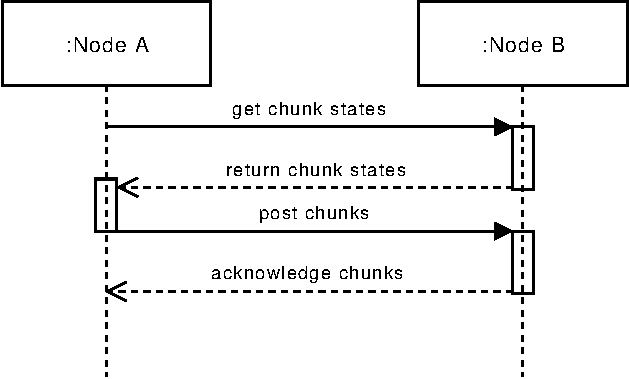
\includegraphics[width=0.6\linewidth]{resources/data_replication.pdf}
    \caption{Data Replication Sequence Diagram}
\end{figure}

This scenario is described in more detail in the appendix \fullref{sec:scenario-data-replication}.

\subsection{Security and Encryption}\label{sec:security-and-encryption}
One of our primary design goals was to ensure that once data is in the redbackup system, it can not be altered or deleted from a \gls{client} to prevent ransomware attacks \cite{young-cryptovirology}. To achieve this, each backup is created with an \gls{expiration-date} on which \glspl{node} are allowed to remove the associated data. Reasoning and potential risks of physical time are discussed in paragraph \fullref{sec:removal-of-old-backups}.

Because \glspl{node} can also be the target of randsomware attacks, each \gls{node}, or its associated \gls{storage} component respectively, must verify that a given data \gls{chunk}s contents are not corrupted using cryptographic hash functions, also known as checksums. To be able to do so, it must be possible to calculate the identifier of such a data \gls{chunk} from its contents. A discussion on the role of hash functions including the chosen algorithms for the study project is carried out in section \fullref{sec:hash-collisions}.

A \gls{client} encrypts backup data \glspl{chunk} when creating a new backup. This ensures that no other participant in the redbackup system can inspect file contents (need-to-know principle \cite{security-patterns}). The encryption and decryption keys are only persisted on the client and must be backed up separately.

All sent \glspl{message} should be signed by the sender. If so, transport layer encryption is not strictly necessary because all user data is already encrypted on the \gls{client} with the only exception of the \gls{expiration-date}.

The \gls{management} component has no knowledge of the persisted data in the system and has only knowledge of the configuration (need-to-know principle \cite{security-patterns}).

A detailed description of these security mechanisms is out of scope for this study project and has to be carried out in the future.

\subsection{Partitioning \& Scaling}

To scale the redbackup system regarding availability and safety more \glspl{node} can be added to the redbackup system. If a given \gls{node} is overloaded, a \gls{client} can use another \gls{node} for its backup creation or restoral. Because both processes require approval of a chosen \gls{node} (See scenarios \fullref{sec:scenario-create-backup} and \fullref{sec:scenario-backup-restore}), an overloaded \gls{node} can finish work in progress backups/restores and reject new requests (following the patterns Finish Work In Progress and Shed Load \cite{fault-tolerance}). The data is replicated to the overloaded \glspl{node} eventually.

We ensured that \glspl{node} are (mostly) stateles which simplifies scaling as well.

Because the proposed system does currently only support \emph{n-replication} (See section \fullref{sec:fundamental-design-decisions}), the maximum storage capacity is the lowest common factor. Therefore, to increase storage capacity, the capacity of all \glspl{node} must be extended to the desired amount.

To minimise network usage deduplication of data is used on the \gls{client}. Deduplication is  discussed in the paragraph Storage Unit in  \fullref{sec:fundamental-design-decisions}.

\subsection{Failure Detection}

Additionally to the above-discussed mechanisms for fault tolerance regarding security and scaling, the following failure detection mechanisms are in place.

Most issues that occur are reported to the \gls{management} component (following the pattern Someone in Charge \cite{fault-tolerance}). The \gls{management} can then decide to notify the system administrator or execute error mitigation processes, e.g. suspend a given \gls{node} temporarily.

If a node tries to connect to another node that is not available, it notifies the management node (following the pattern System Monitor\cite{fault-tolerance}).

Each \gls{node}, or its associated \gls{storage} component respectively, periodically picks $n$ (random) data \gls{chunk} and verifies the persisted contents for possible corruption using the checksum mechanisms discussed in \fullref{sec:security-and-encryption} (following the Pattern Routine Audits \cite{fault-tolerance}). If a corruption is detected, the \gls{storage} notifies the \gls{node} which notifies the \gls{management}.

In case the \gls{management} component is temporarily unavailable, \glspl{node} and \glspl{client} cache configuration data, e.g. which other \glspl{node} exist to perform replication without interruption. Any notifications that were not successfully transmitted to the \gls{management} must be buffered on the \glspl{node} as well to ensure their delivery.

\section{Fundamental Design Decisions}\label{sec:fundamental-design-decisions}

We used the morphological box technique to explore different possible solutions (See Table \ref{tbl:morphological-box})

The chosen option should be as simple as possible for the prototype developed in the study project but extensible for further adaption.

The following paragraphs reason the selected entry in each dimension.

\paragraph{Redundancy}
We originally planned to support \emph{client m-replication}, which means that the client defines a custom degree of redundancy from 1 to the number of nodes. This, however, is a complex mechanism that requires sophisticated algorithms to work correctly and efficiently. For the prototype, we chose the more straightforward to implement option system \emph{n-replication}, where the degree of redundancy for the whole system is equal to the number of nodes in it. Changing this option in the future is hard because it requires fundamental changes in the replication process and the communication protocols.

\paragraph{Storage unit}
The idea of \emph{chunks} come from Borg Backup. Files are partitioned into chunks using a rolling hash which allows deduplication as well as space efficient backups for large files \cite{borg-data-structures}. These are desired properties in a backup system to minimise network and disk usage.

\emph{Encrypting chunks} means that deduplication of the same file coming from different users is not possible anymore but is a necessity for privacy. Encryption is not trivial and requires a user concept that is out of scope of the prototype developed in the study project.
We chose the \emph{plain filesystem} option for the study project to simplify the client implementation. Supporting \emph{encrypted chunks} in the future is possible by just modifying the client.

\paragraph{Role of the management}
The \emph{one in charge} option is the most straightforward option to implement but conflicts with many intentions of the administrator (See \fullref{sec:adminstrator-intention}). We also intended to avoid a single point of failure. We chose the option \emph{autonomous replication} because it guarantees that replication is always ensured and keeps communication relatively simple.

\paragraph{Storage backend}
Using the file system is the simplest possible solution for the study project and therefore selected option. Adding support for other backends in the future is still possible since the storage component is an isolated part of the architecture (See \fullref{sec:component-storage})

The number of files in a folder is limited depending on the used file system, length of a filename and other factors. Some file systems (e.g. ext4) have a global limit for the maximal number of files. This limit is 4 billion files for ext4. \cite{ext4}

We, therefore, use the ext4 file system to persist data in the study project.

\paragraph{Removal of old backups}\label{sec:removal-of-old-backups}
We propose to use a fixed \emph{physical time} that must be specified on backup creation. After expiration, the backup data may be removed by a garbage collector. This may be extended to allow only mutual garbage removal in the future.

A significant problem that \emph{physical time} addresses is the safety of backup data in case a user computer is infected with malware. An illicit application might command the removal of backups, or create new backups to initiate a garbage collection process to free storage capacity.

Nevertheless, the use of \emph{physical time} has the downside of possible data loss due to wrong system times. To lessen this risk, the system should use multiple distinct upstream time-servers. This is given with a high probability, as the proposed redundancy model motivates users to expand the system across multiple physical locations. Furthermore, the client, nodes and management should verify a reasonable accurate time when communicating mutually.

\paragraph{Programming language / ecosystem}
A complete language evaluation can be found in \fullref{sec:language-evaluation}.

\begin{sidewaystable}
	\centering
	\caption[Morphological Box]{Morphological Box}
	\label{tbl:morphological-box}
    \begin{tabu}{X | X X X X}
		\hline
          \textbf{Redundancy}
          & No redundancy
          & Client m-replication: The client defines a custom degree of redundancy (from 1 to the number of nodes).
          & System m-replication: The administrator defines the degree of redundancy for the whole system (from 1 to the number of nodes).
          & \textbf{System n-replication}: The degree of redundancy for the whole system is equal to the amount of nodes in the system.
          \\ \hline

          \textbf{Storage unit}
          & \textbf{Plain files}
          & Encrypted files
          & Chunks: Cut files into multiple parts and store these individually.
          & Encrypted chunks: Same as chunks, but every chunk is individually encrypted.
          \\ \hline


          \textbf{Role of the management}
          & One in charge: The management knows and controls everything (e.g. the location of every file/chunk).
          & Configuration only: The management must be up for administrative tasks only. The nodes are mostly autonomous.
          & \textbf{Autonomous replication}: The management must be available for most of the tasks but replication also works if the management is down.
          & No management: Every node is completely autonomous.
          \\ \hline


          \textbf{Storage backend}
          & \textbf{Plain filesystem}: Just store all files/chunks as files in one directory with a unique identifier.
          & Database: Use an existing database solution (e.g. Git, Redis, RocksDB).
          & Cloud Storage: A proxy to a cloud storage provider (e.g. Amazon S3).
          & Custom: An optimized version of the plain file system option with optimised indexing and compression.
          \\ \hline


          \textbf{Removal of old backups}
          & \textbf{Physical time}: Data is removed on a specified physical time.
          & User command: The user commands removal of data.
          & Free storage: Data is removed, as soon as capacity issues occur.
          & Physical time with mutual agreement: All nodes must agree before data is removed.
          \\ \hline


          \textbf{Programming language / ecosystem}
          & \textbf{Rust}
          & Go
          & Erlang
          & 
          \\ \hline
	\end{tabu}
\end{sidewaystable}

\subsection{Hash Collisions}\label{sec:hash-collisions}
To achieve deduplication and space-efficient backups for large files, as discussed above, a file/chunk identifier must be derived from the actual file/chunk contents. 
A common mechanism used to derive identifiers from binary data are cryptographic hash functions. Most cryptographic hash functions produce a message digest having a fixed size (e.g. SHA-256\cite{sha-256} produces a 256-bit digest) for a message with an arbitrary length, which can theoretically lead to collisions.
Perfect hash functions do not have this property because their input message size is fixed and equal to the size of the resulting message digest. A perfect hash function is not practical in our case due to the large message digests.
With cryptographic hash functions, collisions are possible but unlikely. Assuming that the applied function does produce equally distributed results, the probability can be calculated based on the birthday problem\cite{birthday-attack} as follows, where $p$ is the number of chunks in the system and $n$ the size of the message digests:

\[
P(p, n) = \frac{p^2}{2^{n+1}}
\]

Assuming we have $p=30^{21}$ files/chunks the system (which is equivalent to two billion years of music assuming each chunk has a size of one byte\cite{seagate-zetabyte}) and using the SHA-256 algorithm, the probability of collisions is about $4.72 \cdot 10^{-16}$, which is highly improbable and may therefore be neglected.

If, however, a collision would happen after all, for example, if the used cryptographic hash function is flawed or the unlikely event occurs, it results in data loss.

In theory, we could detect collisions on the client. To do so, every time an identifier is calculated, the client must verify that if a file with the same identifier exists already in the system, it has the exact same contents. If the contents differ, its a collision.This approach requires a lot of network traffic and can slow down the backup process significantly.

Another place to detect collisions is on the node. A node can verify if the contents of a given file/chunk are equal to the contents already present in the system. The downside of this approach is that it requires the client always to send the full contents of every file, which means there is a lot of additional network traffic.

Both of the described approaches for collision detection have significant costs that are not practical.

As for the study project, we use the SHA-256 algorithm\cite{sha-256} and neglect the risk of hash collisions due to its low probability. Nonetheless, we prepare all protocols and components to use an interchangeable mechanism for the calculation and transmission of file/chunk identifiers.

\subsection{Simplifications for the prototype}

Because the whole system as described in the previous sections is too large and complex to implement even in the form of a prototype we reduced the functionality to its core.

Our prototype focused on the backup, restore and replication scenarios as described in appendix \fullref{sec:scenarios}.

We also limited the supported plattforms to 64-Linux only as this is the operating system we use for development and continous integration.

\subsubsection{Concrete Architecture}

Figure \ref{fig:c4-overview} illustrates the system as implemented in our prototype.

The \gls{client} and \gls{node} are delivered as single executables that can are configured and launched using the command line.

The \gls{node} component binds itself to a provided network interface and port on which it provides the services for backup creation, backup restore and replication.

The \gls{client} binary is relaunched for every operation, that is the creation of a backup,  listing all backups persisted on a given \gls{node} and the restoration of data.

All components were implemented using the rust programming language. Installation instructions are documented in the project's repository.

\begin{figure}[h]
	\centering
	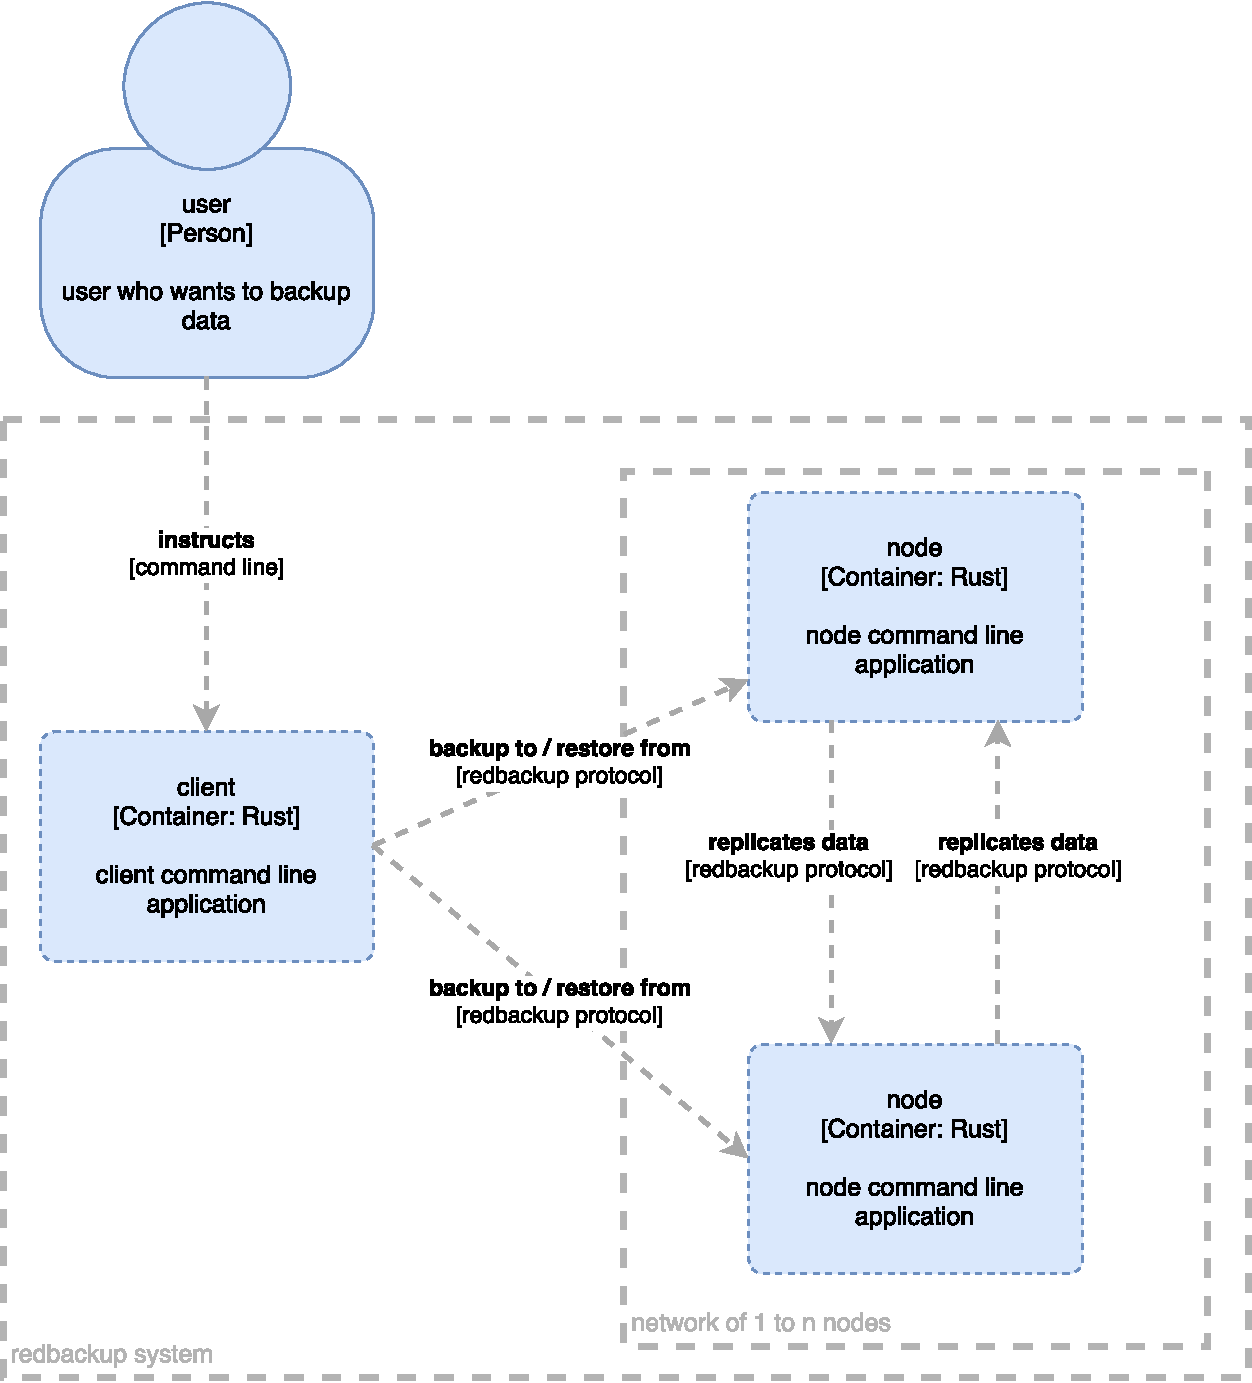
\includegraphics[width=1\linewidth]{resources/c4-sa-container}
	\caption[SA specific C4 Container diagram]{C4 Container diagram illustrating the high-level shape of the prototype and how responsibilities are distributed across it as implemented in the Study Project.}
	\label{fig:c4-sa-container}
\end{figure}

\subsubsection{Client}


The client executable bundles three components as shown in Figure \ref{fig:c4-client-container}. \emph{Client-cli} contains the command line specific logic that provides an uncluttered interface for advanced users and serves as an entry point in the client's core logic. We used the clap\footnote{\url{https://clap.rs/}}  library to implement this component.

\begin{figure}[h]
	\centering
	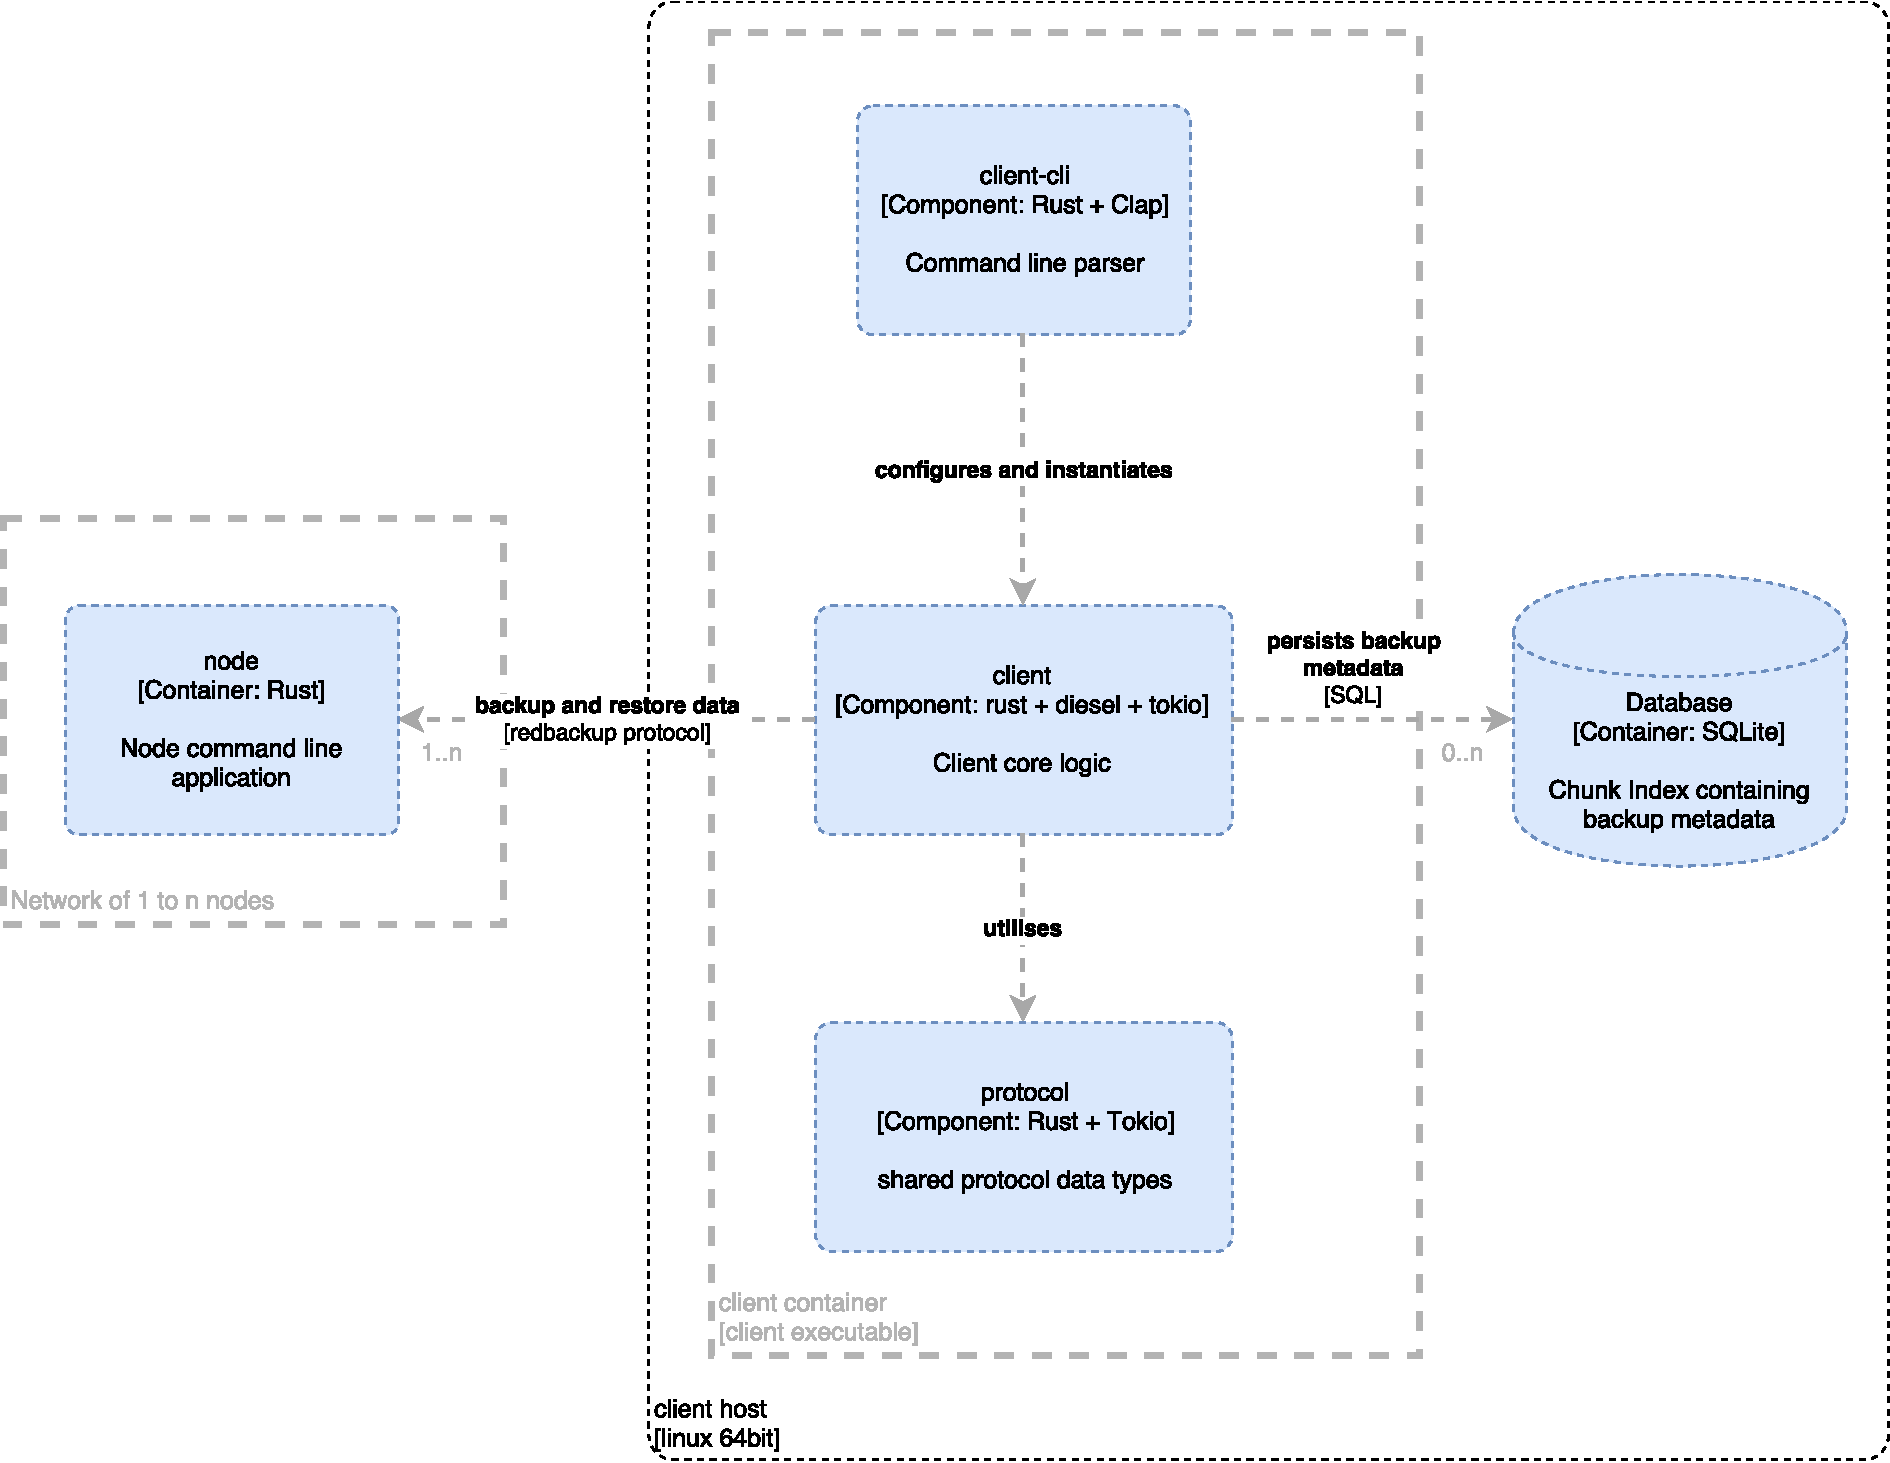
\includegraphics[width=1\linewidth]{resources/c4-client-container}
	\caption[Client specific C4 Container diagram]{C4 Container diagram illustrating the shape of the client and how responsibilities are distributed across it as implemented in the Study Project.}
	\label{fig:c4-client-container}
\end{figure}

The \emph{client} component contains the actual logic for the creation and restoration of backups. It is organised as a library so that it can be used for other projects as well, e.g. if we provide a graphical user interface in the future. The client component creates metadata for every backup in a separate \emph{SQlite-database}. These databases are also the entry point for a restore. For database access, we used the Diesel\footnote{\url{https://diesel.rs/}} ORM-Library.

The \gls{client} components make heavy use of a networking library called tokio \footnote{\url{https://tokio.rs/}} that provides an efficient event loop similar to the Reactor pattern \cite{POSA1}. Although tokio supports highly parallel networking code, we decided to implement all interactions from a \gls{client} to \glspl{node} serial to keep it simple and readable.

The (de-) serialisation mechanisms for messages sent to \glspl{node} are encapsulated in the \emph{protocol} component (Forwarder Receiver Pattern Pattern \cite{POSA1}).

The \gls{node} with which the \gls{client} interacts is passed to the client executable via command line arguments.


\subsubsection{Node}

The node executable bundles four components as shown in Figure \ref{fig:c4-node-container}.  

\begin{figure}[h]
	\centering
	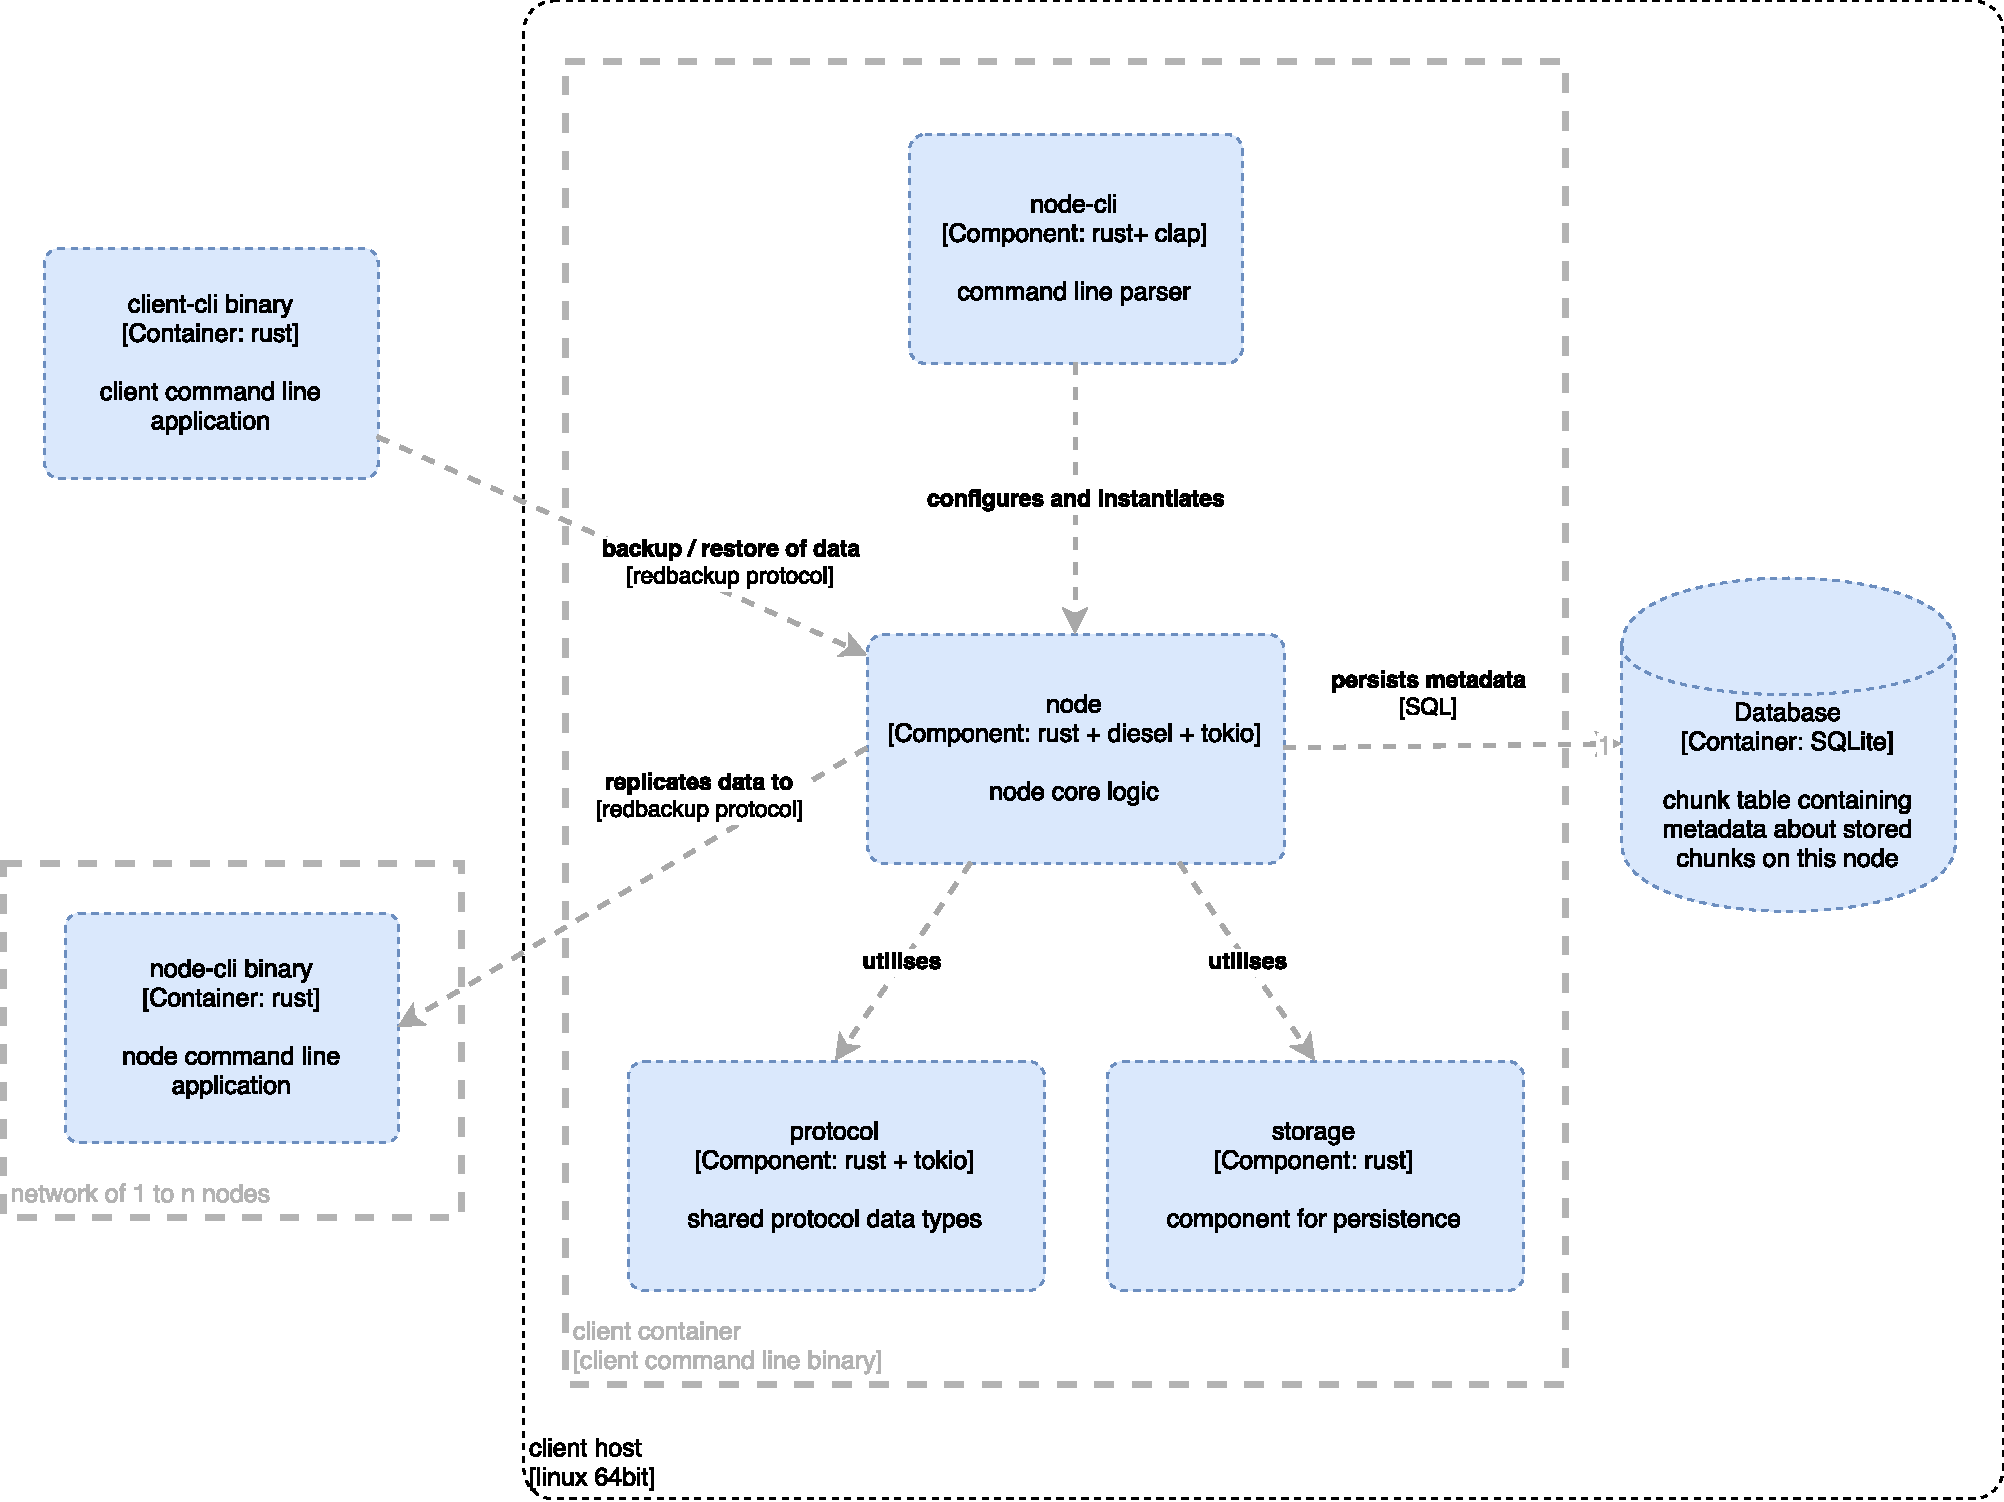
\includegraphics[width=1\linewidth]{resources/c4-node-container}
	\caption[Node specific C4 Container diagram]{C4 Container diagram illustrating the shape of the node and how responsibilities are distributed across it as implemented in the Study Project.}
	\label{fig:c4-node-container}
\end{figure}

Analogous to the client implementation, the command line logic is encapsulated in a separate component called \emph{node-cli}.

The core logic is implemented in the \emph{node} library. Like the client, the node component makes heavy use of the tokio and Diesel library. In contrast to the client, we used the parallel features of tokio. To keep the chosen technology as close to the client, we decided to use SQLite to store metadata about the data \glspl{chunk} present on the node as well. This must be changed in the future because SQLite locks the entire database when writing which makes concurrent updates impossible \cite{sqlite-locking}.

We use the same \emph{protocol} component for (de-) serialisation of messages on the node and the client.

The \emph{storage} component is also bundled directly in the node executable. It persists data in one single directory as described in \fullref{sec:fundamental-design-decisions}.

Other known nodes are passed to the node executable via command line arguments.

Because user authentication is complex and requires additional cryptographic efforts, the prototype accepts backups and replications from everyone.

\section{Testing}\label{testing}

In the following chapters we illustrate, how we tested our prototype and architecture.

\subsection{Unit Tests}\label{unit-tests}
We used test driven development (TDD) to develop the prototype as much as possible. Our Definition of Done\cite{project-plan} states that \emph{reasonable unit and integration tests [must] exist and pass.}

Therefore, all unit tests were executed on every build run of our continuous integration, that is on every repository push and pull request.

Some unit tests written for the prototype are not pure unit tests but minimal integration tests. Because Rust is not a traditional object-oriented language, it is not possible to introduce and use interfaces (Traits) in the same way as we were used to from other languages such as Java or C#. Due to the steep learning curve Rust has, we were not able to fully utilise the corresponding mechanisms. 

\subsection{Integration Tests}\label{integration-tests}

Our integration tests are split into two main environments: A minimal one as defined in Figure \ref{fig:integrationtestsmall} and a medium network, as defined in Figure \ref{fig:integrationtestmedium}.

\begin{figure}
	\centering
	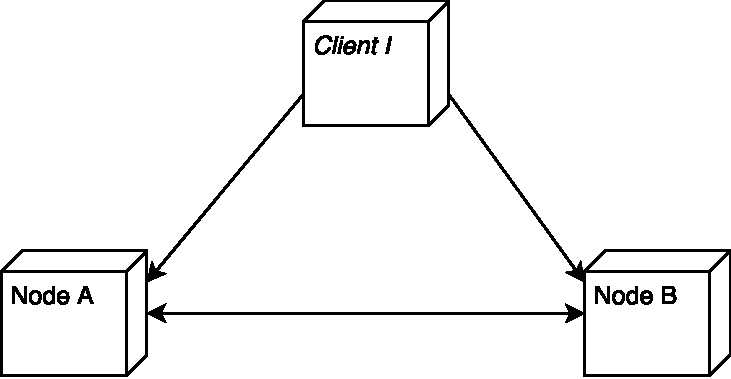
\includegraphics[width=0.5\linewidth]{resources/integration_test_small}
	\caption[Minimal integration test]{Minimal integration test with one client and two nodes.}
	\label{fig:integrationtestsmall}
\end{figure}

\begin{figure}
	\centering
	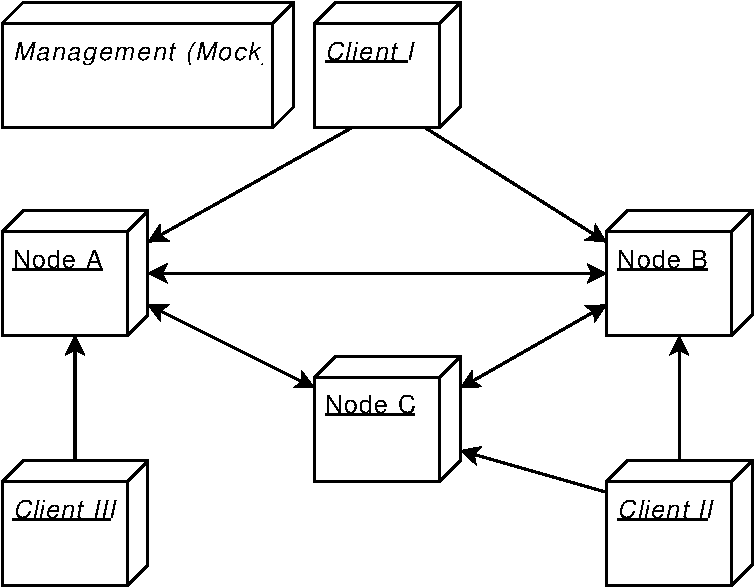
\includegraphics[width=0.5\linewidth]{resources/integration_test_medium}
	\caption[Medium integration test]{Medium integration test with three clients and three nodes.}
	\label{fig:integrationtestmedium}
\end{figure}

These two, rather small network styles will probably be the most commonly used deployments, yet cover most of the possible problems that may occur.

The integration tests are run automatically at least on every tagged release (i.e. at least once every sprint). Because of the (yet) small set of integration tests we created in the prototype, we ran the tests on every build.

To write integration tests as effective as possible, we created a testing library written in python that enabled us to write comprehensive black box tests. In this framework, the internals on how to launch and configure clients and nodes is encapsulated in classes. Using this abstraction, we decided to launch clients and nodes in separate docker containers, so that they are as isolated as possible. All containers used in a test case are connected to a dedicated docker network which eliminates possible interferences with other network services.

We wrote integration tests that verify that a backup can be created, is replicated onto other nodes and is restored flawlessly.

Tests for the fault tolerance, e.g. what happens if a node goes down during a backup, canb be implemented as integration tests as well.

\subsection{Test coverage}

Since Rust is still a young language with a relatively small ecosystem, tools for measuring code quality are still rare and immature. For our unit tests, we used Tarpaulin \footnote{\url{https://github.com/xd009642/tarpaulin}} to generate code coverage. Tarpaulin does not (yet) cover all language features and therefore returns a conservative coverage number. We achieved 53.5\% line coverage taking into account that this number would be significantly higher if all executed lines were counted (e.g. generated code using macros as well as compiler optimisations such as the removal of else statements are not counted).
Code coverage achieved using the integration tests is not yet supported by any tool known to us and therefore undocumented. The integration tests do however cover all positive scenarios that were implemented.

\subsection{Architecture tests}

Architectural tests are special, manually run tests to verify the scalability of our software architecture.

Our integration testing framework allowed us to write such tests in a simple fashion.

\subsubsection{Size scalability}
As per our requirements in Appendix \ref{requirements}, the architecture should scale up to 100 nodes. To test this scenario, we use the same underlying techniques as in our integration tests (see chapter \ref{integration-tests}), but scale the infrastructure up to the required limits.

Due to the high memory consumption of our prototype, we were not able to conduct this test with a significant amount of data. We conducted one test, in which a file of 5MB was replicated to 99 Nodes which worked just fine.

\subsubsection{Data capacity}
Our requirements (Appendix \ref{requirements}) also state, that a node must be able to handle up to e.g. 2TB of data. To test this requirement, we planned to create large amounts of random data that has to be stored. This is a realistic requirement, as e.g. a compressed image, audio and movie collection might reach such sizes in practice.

Both, the client and the server of the prototype use lots of memory during the creation of a backup. It was therefore not possible yet to create a single backup of 2TB. Performing multiple backups in a row of a smaller dataset (i.e. 5 files with a size of 500MB) did not show any sign of a decreasing performance.

\subsubsection{Concurrent Backups}

We ran a test in which 5 clients back up randomly generated data onto three randomly chosen Nodes. On average, the complete backup process of 1MB of data took 90-130ms from one docker container into another. In reality where clients and nodes are on separate physical machines this time will be higher of course.

These test are however somewhat problematic because the creation of backups require lots of CPU power for the calculation of hashes. Running all clients on separate machine might would probably improve the performance slightly.



\section{TODO}

\begin{itemize}
	\item we never discuss root handles and the conenction to SQLite databases.
	\item should we reference the C4 model somewhere?
\end{itemize}